\documentclass{article}
\usepackage{graphicx} % Required for inserting images
\usepackage{IEEEtrantools}

\title{Tarea 1 Bases de Datos: Modelación de diagrama ER para TCG Pokemon.}
\author{Miguel Enrique Soria Centeno - A01028033}
\date{Abril 2024}

\begin{document}

\maketitle

\section{Introducción}
El siguiente documento tiene como objetivo modelar un diagrama Entidad-Relación para un sistema de base de datos que almacene información de cartas de un juego de cartas coleccionables (TCG) de Pokemon, y explicar las relaciones mostradas entre las tablas en el contexto del juego. 

\section{Modelo ER}
\begin{center}
  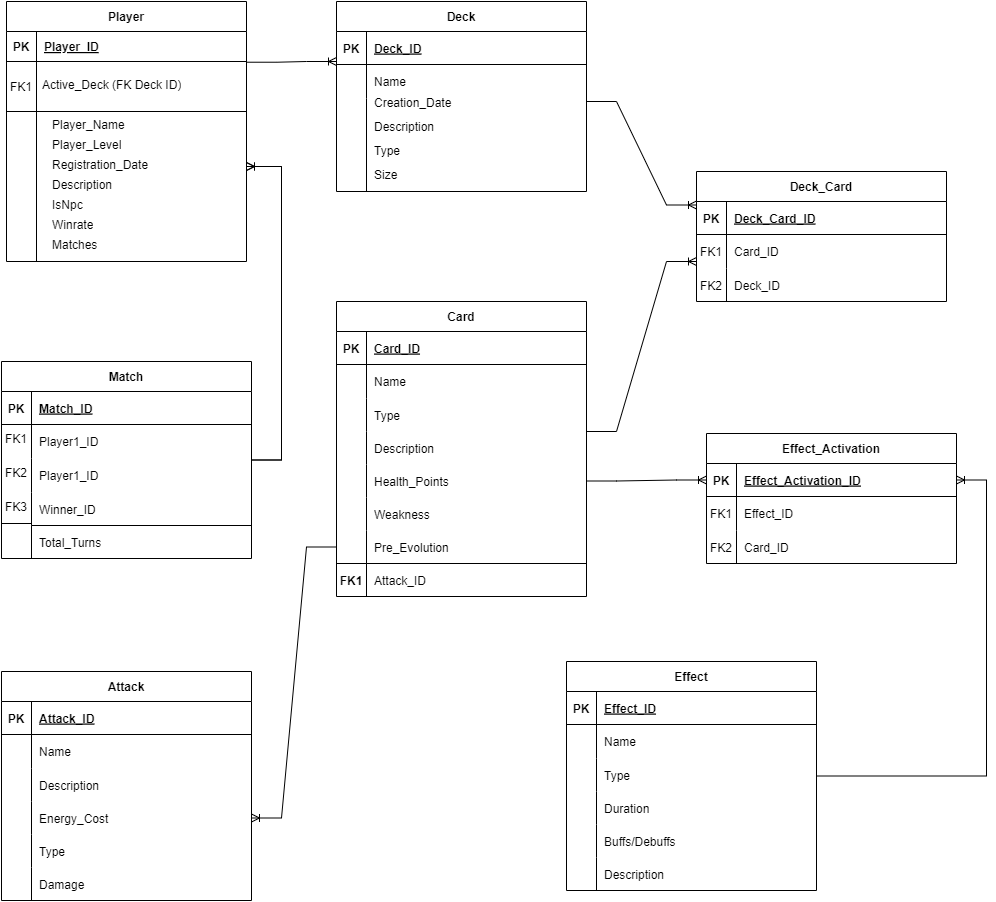
\includegraphics[width=0.8\textwidth]{PokemonTCG_ER.png}
\end{center}

\section{Explicación de Entidades y Relaciones}

\begin{itemize}
  \item \textbf{Player:} \textit{Active\_Deck} es una llave foránea con referencia a \textit{Deck}. Los demás atributos son valores del usuario o jugador. 
  \item \textbf{Deck\_Card:} \textit{Deck\_ID, Card\_ID} son llaves foráneas que hacen referencia a las entidades \textit{Deck} y \textit{Card} respectivamente. Un mazo puede tener múltiples cartas, y una carta puede estar en múltiples mazos. Esta tabla es una tabla intermedia conectando la relación muchos a muchos entre \textit{Deck} y \textit{Card}. 
  \item \textbf{Match:} \textit{Player1\_ID, Player2\_ID, Winner\_ID} son llaves foráneas que hacen referencia a la entidad \textit{Player}. Un partido tiene dos jugadores y un ganador. Esta relaci\'on es de uno a muchos. 
  \item \textbf{Card:} Esta entidad almacena informaci\'on de las cartas del juego. \textit{Card\_ID} es la llave primaria. \textit{Attack\_ID} es una llave foránea que hace referencia a la entidad \textit{Attack}, conteniendo la ionformaci\'on de los ataques de la carta. La relacion de \textit{Card} con \textit{Attack} es de uno a muchos. 
  \item \textbf{Effect\_Activation:} \textit{Card\_ID, Effect\_ID} son llaves foráneas que hacen referencia a las entidades \textit{Card} y \textit{Effect} respectivamente. Una carta puede tener múltiples efectos, y un efecto puede estar en múltiples cartas. Esta tabla es una tabla intermedia conectando la relación muchos a muchos entre \textit{Card} y \textit{Effect}. 
  \item \textbf{Effect:} Esta entidad almacena informaci\'on de los efectos de las cartas. \textit{Effect\_ID} es la llave primaria.

\end{itemize}
\end{document}
